%!TEX root = skripsi.tex

\addChapter{Lampiran 1 : Panduan Evaluasi \textit{Word Alignment}}

%\chapter*{Lampiran 1 : Panduan Evaluasi \textit{Word Alignment}}

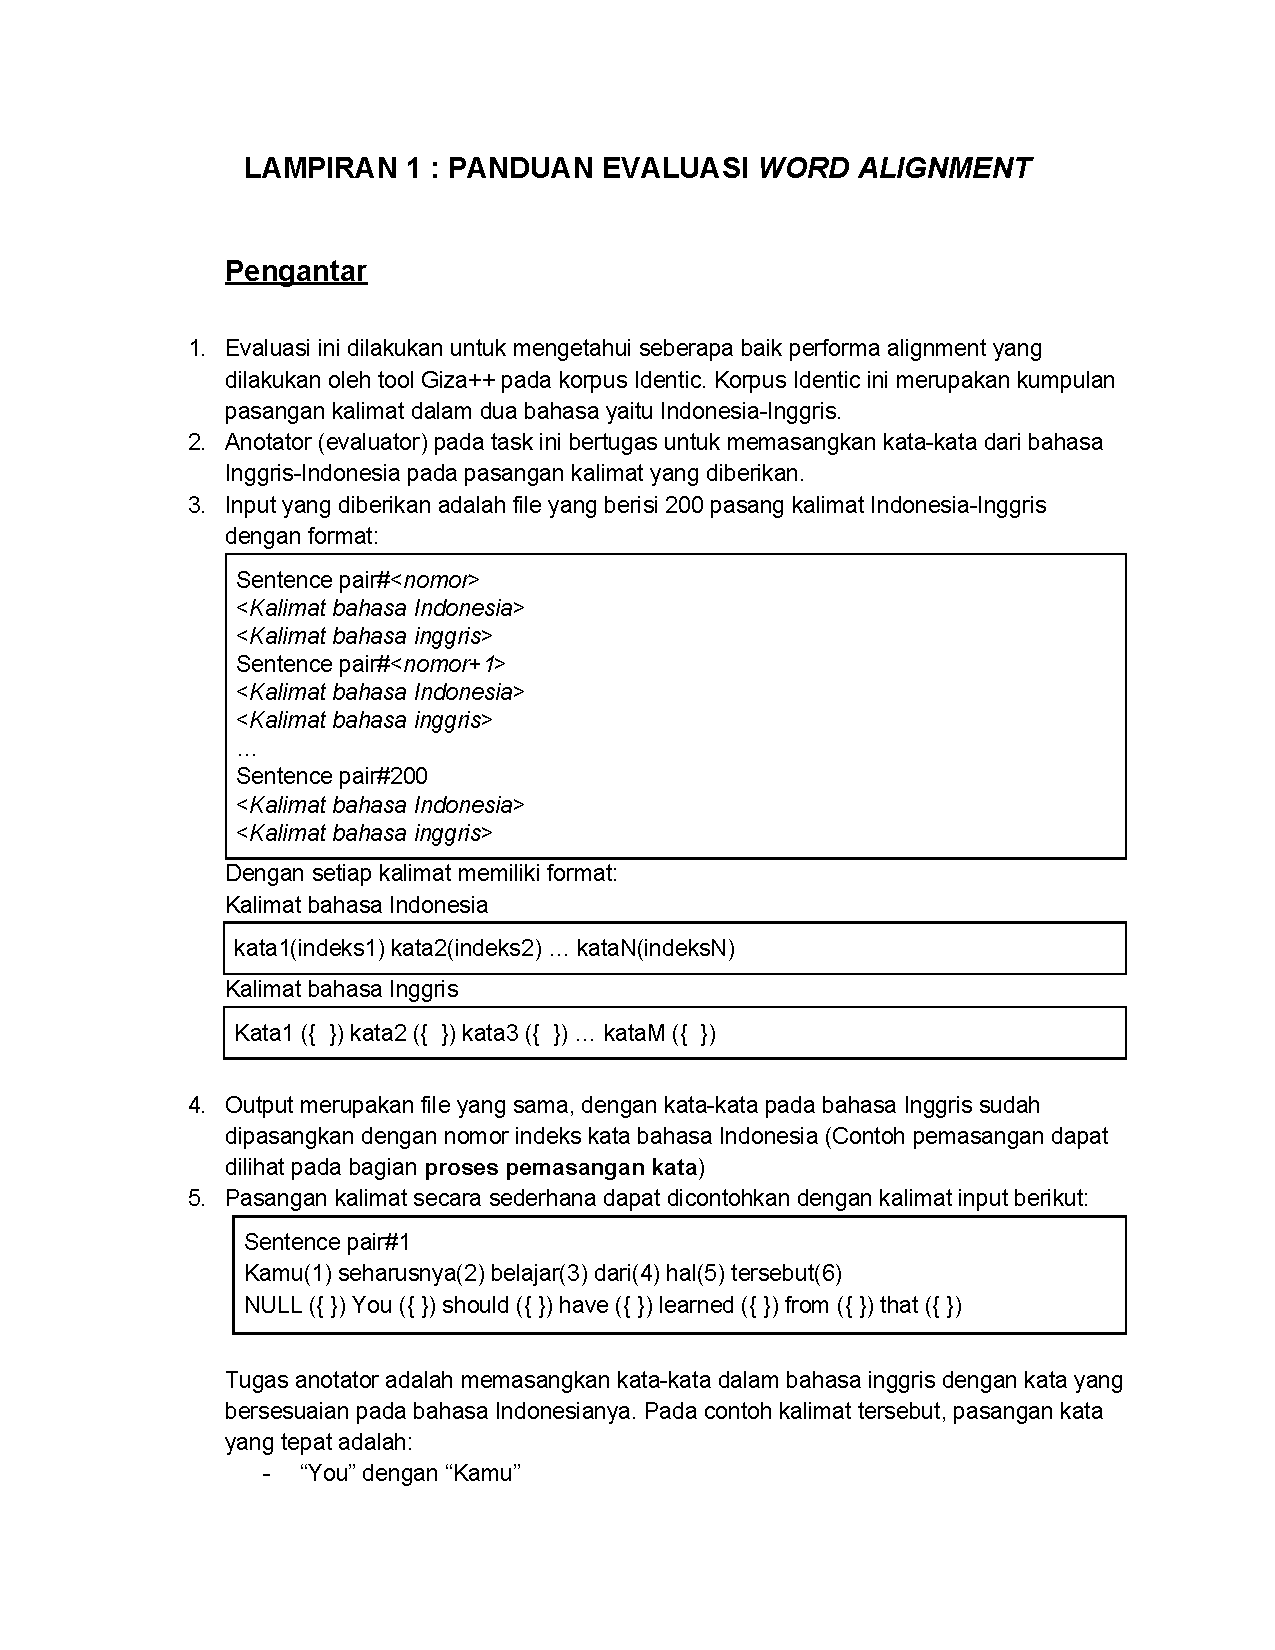
\includepdf[pages={-}, pagecommand={}]{pewa_2.pdf}

\begin{comment}


\section*{Pengantar}

\begin{enumerate}
	\item Evaluasi ini dilakukan untuk mengetahui seberapa baik performa alignment yang dilakukan oleh tool Giza++ pada korpus identik. Korpus identik ini merupakan kumpulan pasangan kalimat dalam dua bahasa yaitu Indonesia-Inggris.
	\item Anotator (evaluator) pada task ini bertugas untuk memasangkan kata-kata dari bahasa Inggris-Indonesia pada pasangan kalimat yang diberikan.
	\item Input yang diberikan adalah file yang berisi 200 pasang kalimat Indonesia-Inggris dengan format:
\begin{lstlisting}[backgroundcolor = \color{white}]
Sentence pair#< nomor >
< Kalimat bahasa Indonesia >
< Kalimat bahasa Indonesia >
Sentence pair#< nomor+1 >
< Kalimat bahasa Indonesia >
< Kalimat bahasa inggris >
...
Sentence pair#200
< Kalimat bahasa Indonesia >
< Kalimat bahasa inggris >
\end{lstlisting}
	Dengan setiap kalimat memiliki format:\\
	Kalimat bahasa Indonesia
\begin{lstlisting}[backgroundcolor = \color{white}]
kata1(indeks1) kata2(indeks2) ... kataN(indeksN)
\end{lstlisting}	
Kalimat bahasa Inggris
\begin{lstlisting}[backgroundcolor = \color{white}]
Kata1 ({ }) kata2 ({ }) kata3 ({ }) ... kataM ({ })
\end{lstlisting}
	\item Output merupakan file yang sama, dengan kata-kata pada bahasa Inggris sudah dipasangkan dengan nomor indeks kata bahasa Indonesia (Contoh pemasangan dapat dilihat pada bagian \textbf{proses pemasangan kata})
	\item Pasangan kalimat secara sederhana dapat dicontohkan dengan kalimat input berikut:
\begin{lstlisting}[backgroundcolor = \color{white}]
Sentence pair#1
Kamu(1) seharusnya(2) belajar(3) dari(4) hal(5) tersebut(6)
Kamu(1) seharusnya(2) belajar(3) dari(4) hal(5) tersebut(6)
\end{lstlisting}
	Tugas anotator adalah memasangkan kata-kata dalam bahasa inggris dengan kata yang bersesuaian pada bahasa Indonesianya. Pada contoh kalimat tersebut, pasangan kata yang tepat adalah:
	\begin{enumerate}
		\item 'You' dengan 'kamu'
		\item 'should' dengan 'seharusnya'
		\item 'learned' dengan 'belajar'
		\item 'from' dengan 'dari'
		\item 'that' dengan 'hal tersebut'
	\end{enumerate}
\end{enumerate}

\section*{Proses Pemasangan Kata}
\begin{enumerate}
	\item Diberikan pasangan kalimat dalam bahasa Inggris dan bahasa Indonesia sebanyak 200 buah pasangan:\\
	contoh \textbf{input} pasangan 1:
	
\end{enumerate}

\end{comment}